\section{Benchmarking \irace}
Given that \irace has not being applied to tackle \nasbench, we study its performance with different setups for a fair comparison with the other \nasbench techniques. We note that when dealing with known benchmarks, ACs can benefit from tailored setups as they can exploit known characteristics of the benchmarks.

\leslie{}{NOTE: I would suggest to omit the experiments with fixed number of configurations and also the ones that set the configuration budget as number of experiments, as they are not the best performing and it might simplify the analysis.}

We performed 20 repetitions of \irace setting 10 million TPU seconds as total configuration budget and evaluate the performance obtained by the following setup options:

\begin{description}[style=unboxed, leftmargin=0px]
\item[Estimation budget] Budget assigned for the initial estimation of the average execution time of an evaluation. We perform experiments with 2\% and 0.2\% of the total configuration time for budget estimation.
\item[First test] Number of evaluations required to perform the first elimination test in a race. We perform experiments with 2 and 3 evaluations for applying the initial test.
\end{description}

For further details of these setup options we refer to~\cite{LopDubPerStuBir2016irace}. Figure~\ref{fig:irace-performance} gives the ECDFs of the final quality obtained by the different setups of \irace. The best overall performance is obtained by setting the estimation budget to $2\%$ of the total configuration time and allowing 3 evaluations before the first elimination test (mean test regret $0.002837$).
\begin{figure}[!t]
\centering
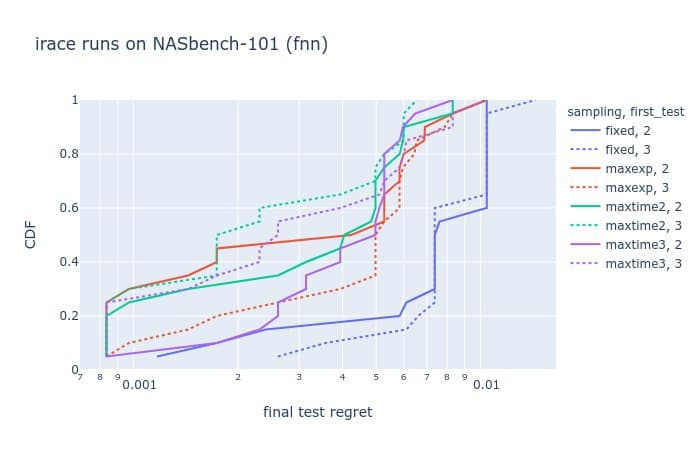
\includegraphics[width=\linewidth, clip=true, trim=30px 35px 0px 50px]{imgs/fnn-irace.png}
\caption{Empirical cumulative distribution function~($x$-axis) of the final regret~($y$-axis) from 20 runs of each \irace setup.}
\label{fig:irace-performance}
\end{figure}
